\section{Manuel utilisateur}
Dans cette partie on vous expliquera comment profiter de site PariService en décrivant le manuel d'utilisation des fonctionnalités proposés. 
\subsection{L'obtention d'un profil}
Pour utiliser les services proposées par le site PariServices, vous allez besoin d'une compte utilisateur et pour l'obtenir on appuie sur le bouton \textbf{Créer un compte} et on remplit la formulaire comme ci-dessous.\newline

\begin{minipage}{0.53\textwidth}
	\begin{figure}[H]
		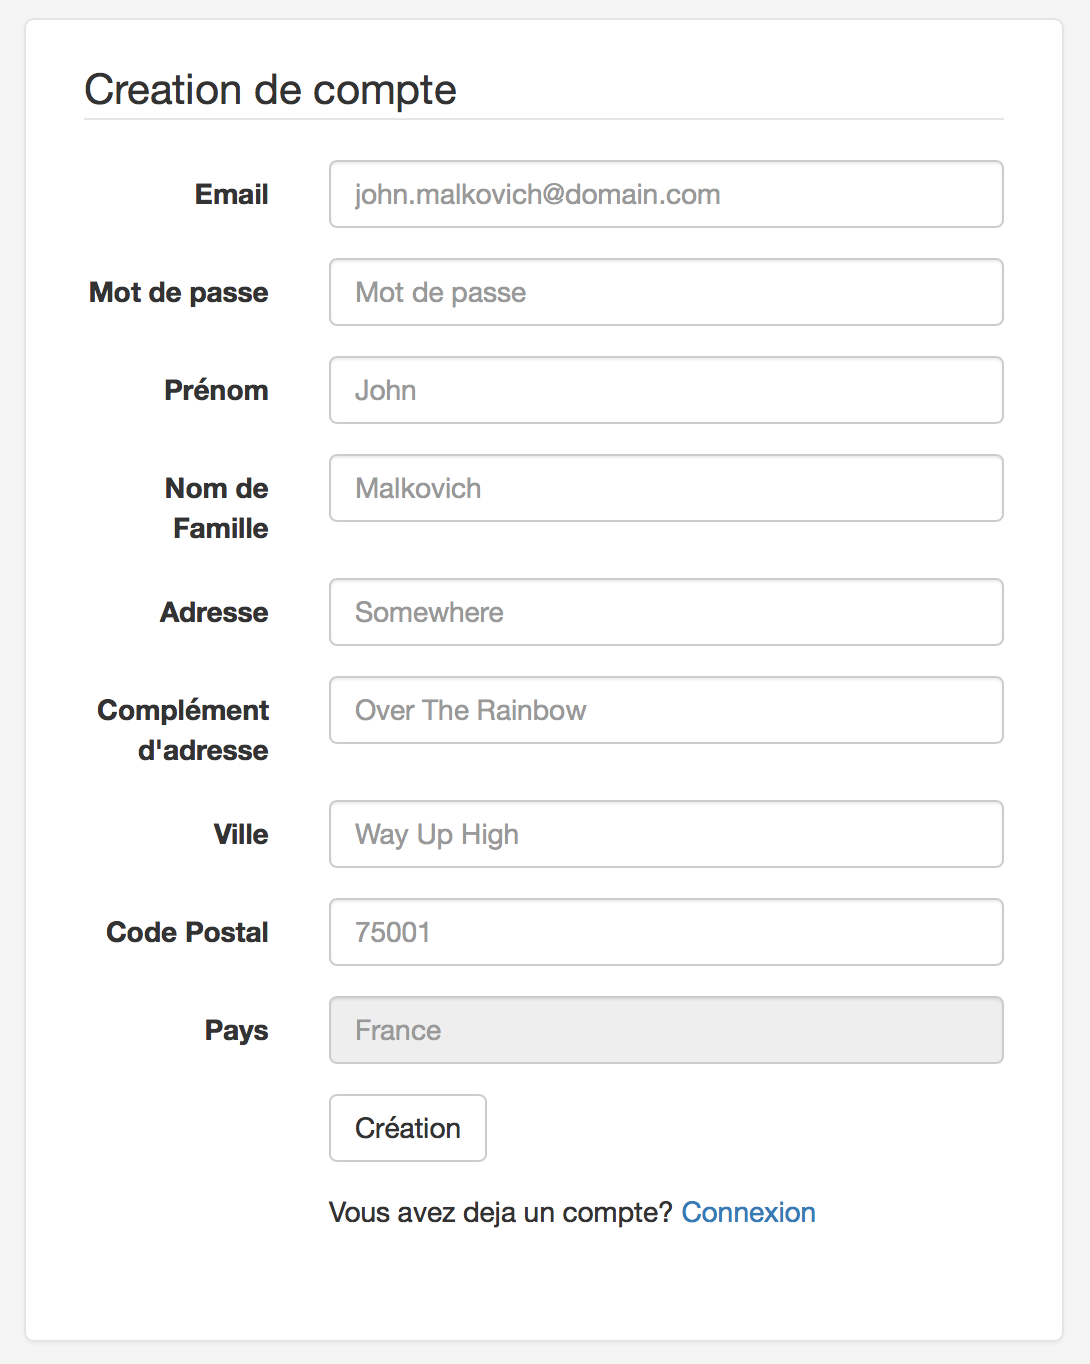
\includegraphics[width=1\textwidth]{images/manuel/signup}
		\caption{Page d'inscription \label{overflow}}
	\end{figure}
\end{minipage} \hfill
\begin{minipage}{0.45\textwidth}
\subparagraph{Inscription.}Après avoir rempli la forme correctement avec un bouton \textbf{Création} on sera redirigé sur la page principale de \textbf{\textit{PariServices}}, sinon les erreurs correspondants seront affichés.\newline
\subparagraph{Authentification.} Dans le cas où vous avez déjà un compte, vous pouvez l'accéder en entrant votre mail et mot de passe sur la page d'authentification.
\begin{figure}[H]
	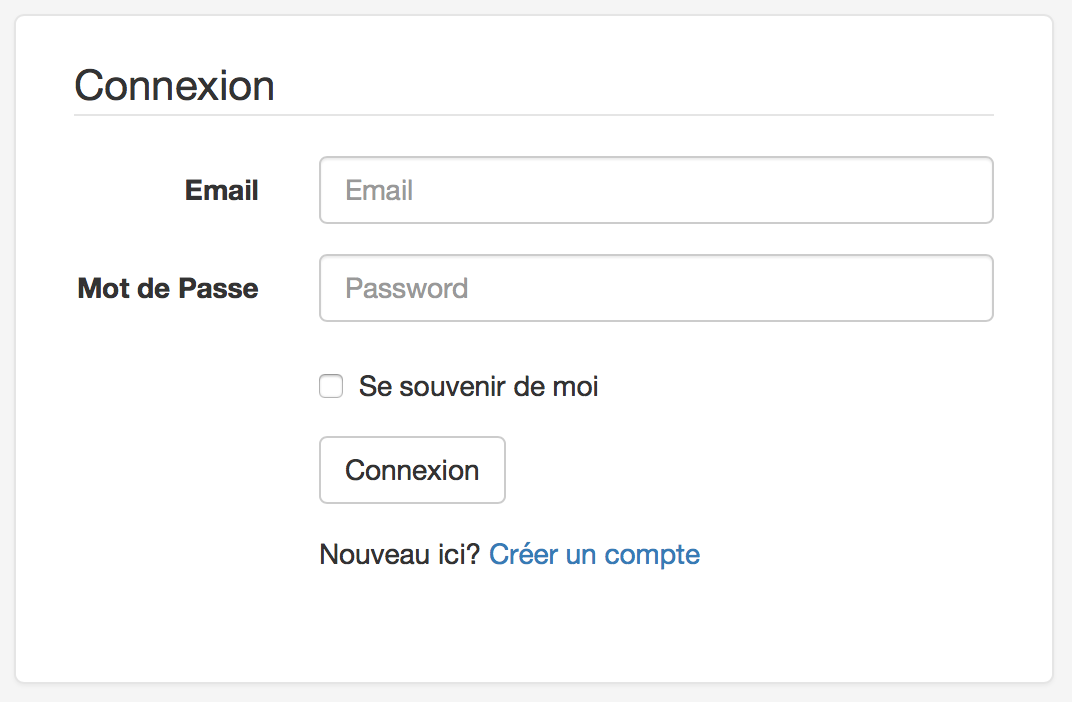
\includegraphics[width=1\textwidth]{images/manuel/signin}
	\caption{Authentification \label{overflow}}
\end{figure}
\end{minipage}\\\\\\

La page principale vous propose de choisir parmi les actions suivantes: \textbf{Rendre un service}, \textbf{Demander un service}, \textbf{Gestion de la profile} et \textbf{Déconnexion}.

\newpage
\subsection{La gestion d'un profil}
La page de profile d'utilisateur nous propose 5 onglets différents:

\subparagraph{Informations} visualise nos informations personnelles.

\begin{figure}[H]
	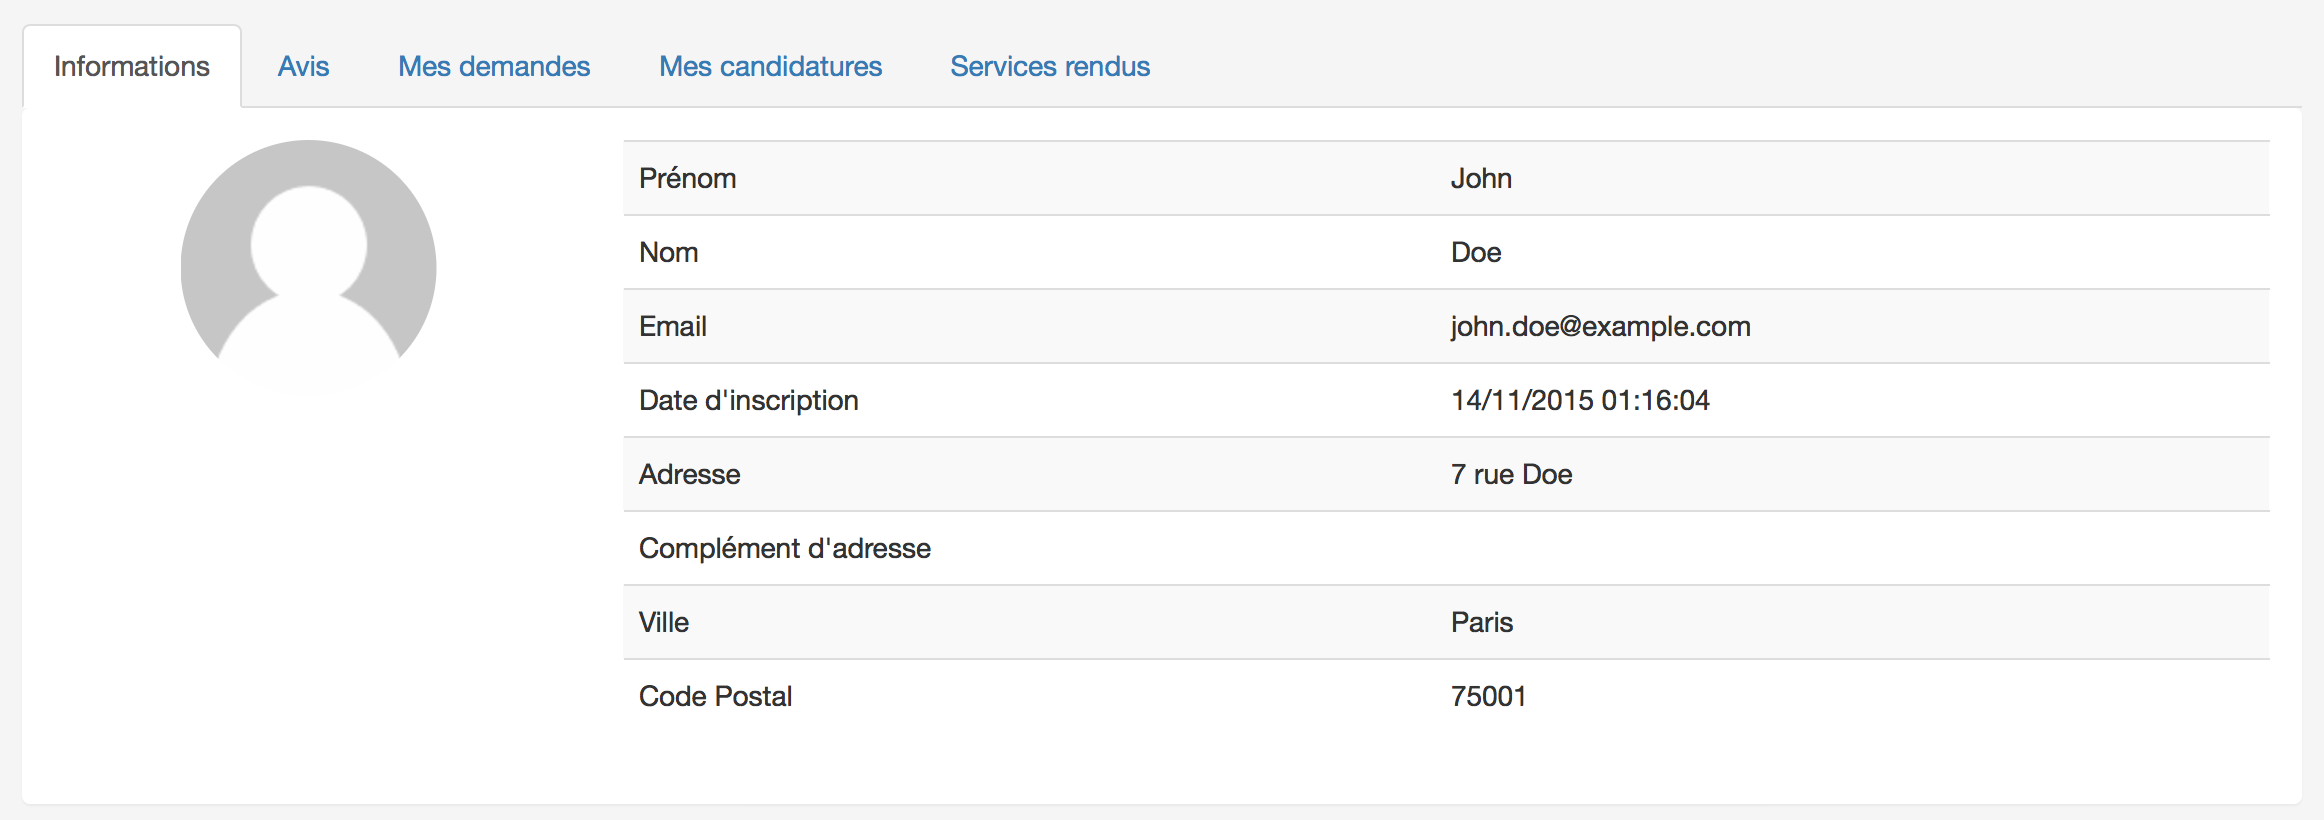
\includegraphics[width=1\textwidth]{images/manuel/profile}
	\caption{Page de la profile \label{overflow}}
\end{figure}

\subparagraph{Avis:} Les évaluations laissés par d'autre utilisateurs qui ont déjà rendu des services pour vous ou pour qui vous avez rendu des services.

\subparagraph{Mes demandes} affiche la liste des services qu'on a annoncé.

\subparagraph{Mes candidatures} affiche la liste des services sur lesquels on a présenté  notre candidature.
\subparagraph{Services rendus} affiche la liste des services qui sont déjà terminé et dans lesquels on a participé soi comme demandeur soit comme candidat.

\subsection{Demander un service}
\begin{minipage}{0.50\textwidth}
	Voici la forme à remplir pour demander un service. Essayer de bien remplir cette forme pour que gens puisse s'intéresser de votre annonce . Aussi c'est très important de correctement spécifier la catégorie et des tags car cela permet aux utilisateurs filtrer et chercher des annonces qui peuvent les intéresser. Après la date spécifié dans \textbf{Fin des candidatures} votre annonce sera automatiquement terminé et plus visible pour d'autres utilisateurs.
	\indent\paragraph{} Appuyer  sur \textbf{Submit} pour placer votre demande sur PariServices.
\end{minipage} \hfill
\begin{minipage}{0.45\textwidth}
	\begin{figure}[H]
		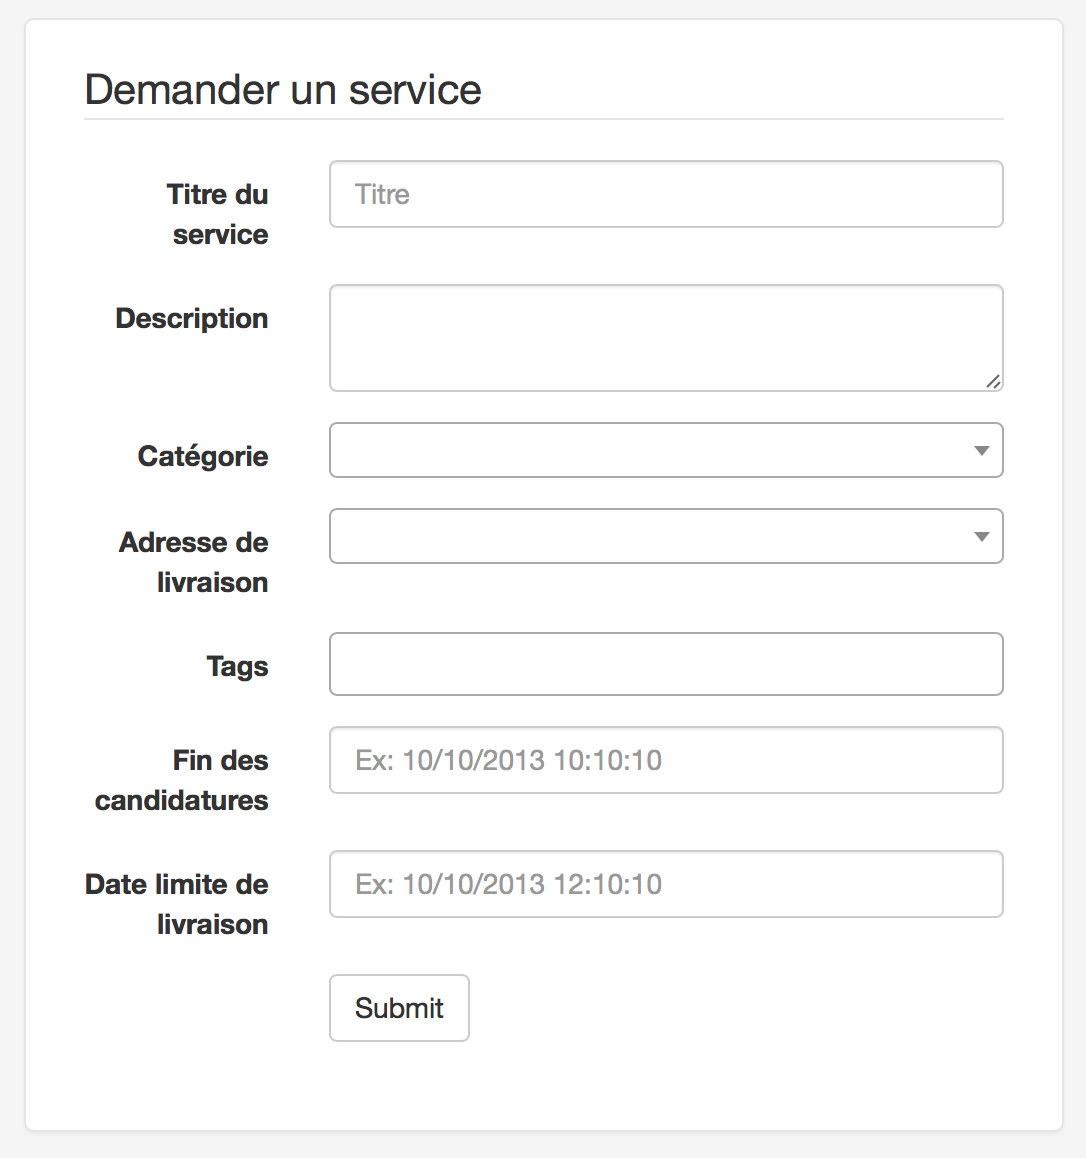
\includegraphics[width=1\textwidth]{images/manuel/demander}
		\caption{Page d'inscription }
	\end{figure}
\end{minipage}\\\\\\


\subsection{Rendre un service}
La page de \textbf{Rendre un service} contient bar de recherche (\textit{Figure ~\ref{fig:recherche}}) et la liste des résultats correspondant à les critères de recherche. Sur la \textit{Figure ~\ref{fig:resultat}} on voie une exemple de recherche avec un tag "New tag" et la liste des résultats contient une annonce nommée "New Example". 

\begin{figure}[H]
	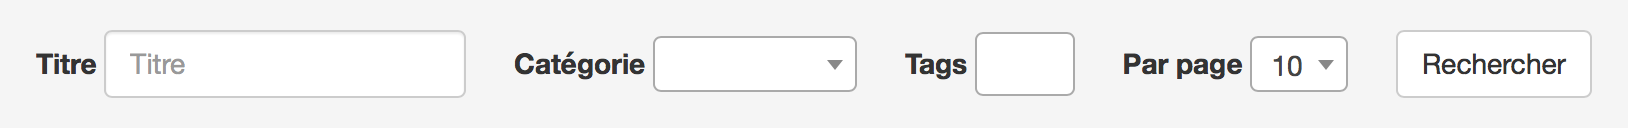
\includegraphics[width=1\textwidth]{images/manuel/recherche}
	\caption{Bar de recherche }
	\label{fig:recherche}
\end{figure}
\begin{figure}[H]
	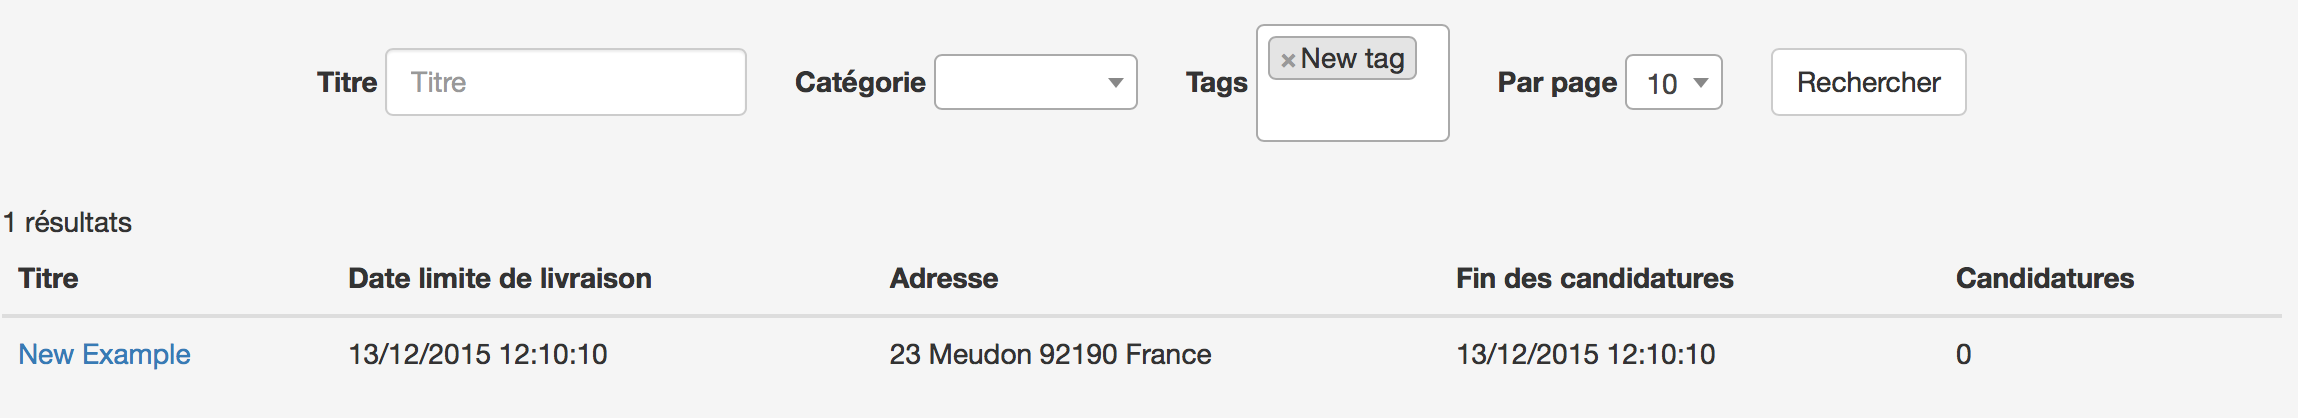
\includegraphics[width=1\textwidth]{images/manuel/resultat}
	\caption{Résultats de recherche }
	\label{fig:resultat}
\end{figure}

\paragraph{}
En appuyant sur le nom de demande on peut visualiser l'annonce qui contient 3 parties principales: 
\begin{enumerate}
	\item Informations sur (\textit{Figure ~\ref{fig:infoannonce}})
	\begin{itemize}
		\item demandeur
		\item description de l'annonce
		\item adresse de rendez-vous
	\end{itemize}
	\item La forme à remplir pour visualiser le chemin optimal de notre adresse vers l'adresse de rendez-vous.  (\textit{Figure ~\ref{fig:formeadresse}})
	\item La carte Google Maps
\end{enumerate}

\begin{figure}[H]
	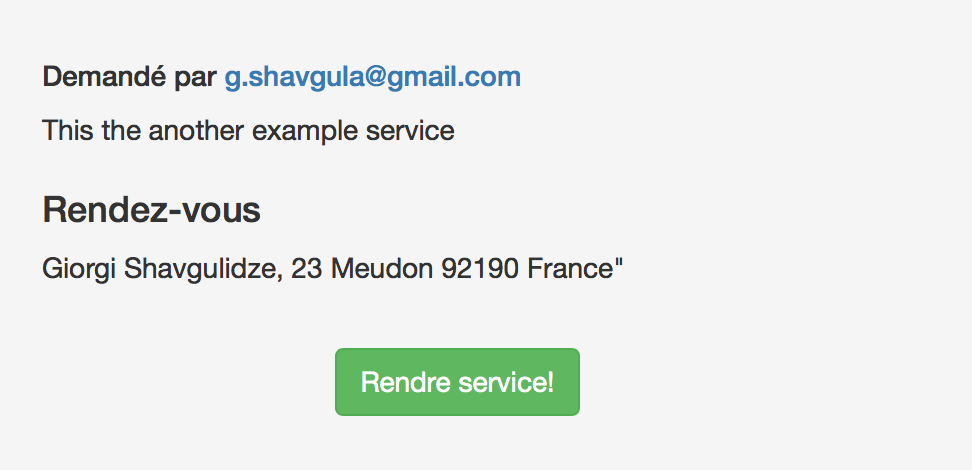
\includegraphics[width=1\textwidth]{images/manuel/demandeur}
	\caption{Informations sur demandeur \& annonce }
	\label{fig:infoannonce}
\end{figure}
\begin{figure}[H]
	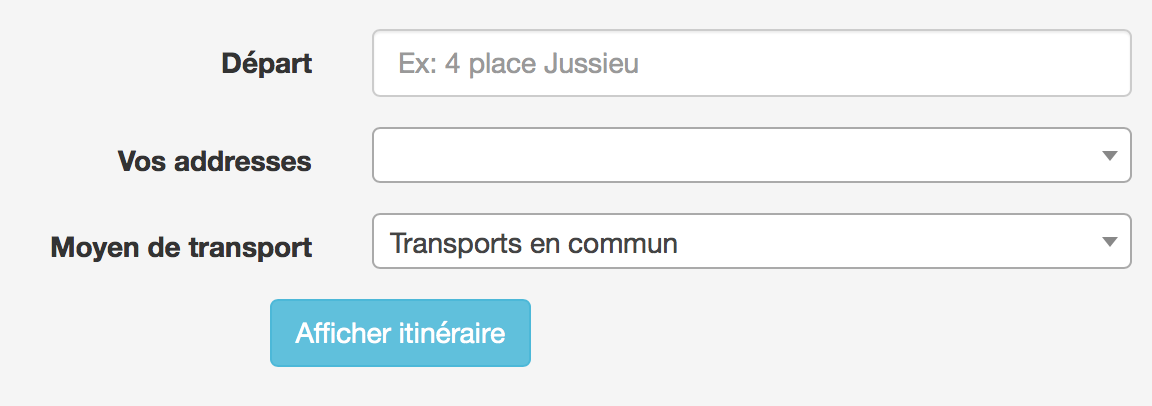
\includegraphics[width=1\textwidth]{images/manuel/adresse}
	\caption{Comment y arriver? \label{overflow}}
	\label{fig:formeadresse}
\end{figure}

\pagebreak

\subsection{Interface}
Ici sera la description de l'interface...
\subsection{Case d'utilisation}
Ici sera la description des cas d'utilisation...
